\documentclass{beamer}
\usepackage{alltt}
\usepackage{tikz}
\usetikzlibrary{matrix}
\usetikzlibrary{trees}
\usepackage{cancel}
\usepackage{subcaption}
\PassOptionsToPackage{obeyspaces}{url}
\usepackage{hyperref}
\usepackage{adjustbox}

\usepackage{lipsum}

\usetheme{Hannover}

\newcommand{\racket}{\texttt{Racket}}
\newcommand{\drr}{\texttt{DrRacket}}
\newcommand{\fsm}{\texttt{FSM}}
\newcommand{\ide}{\texttt{IDE}}
\newcommand{\api}{\texttt{API}}
\newcommand{\arrow}{\(\rightarrow\)}
\newcommand{\dotss}{\(\ldots\)}
\newcommand{\vdotss}{\(\vdots\)}
\newcommand{\elist}{\texttt{\textquotesingle{()}}}
\newcommand{\logand}{\texttt{\(\wedge\)}}
\newcommand{\logor}{\texttt{\(\vee\)}}
\newcommand{\imp}{\texttt{\(\Rightarrow\)}}
\newcommand{\sig}{\texttt{\(\Sigma\)}}
\newcommand{\delt}{\texttt{\(\delta\)}}
\newcommand{\sigsig}{\texttt{\(\Sigma\) = \{a b\}}}
\newcommand{\gam}{\texttt{\(\Gamma\)}}
\newcommand{\ep}{\texttt{\(\epsilon\)}}
\newcommand{\quot}{\texttt{\textquotesingle{}}}
\newcommand{\dquot}{\texttt{"}}
\newcommand{\qquot}{\texttt{\textasciigrave{}}}
\newcommand{\lambexpr}{\texttt{$\lambda$}-expression}
\newcommand{\lamb}{\texttt{$\lambda$}}
\newcommand{\is}{\texttt{::=}}

\definecolor{darkgreen}{RGB}{102,170,102}

\begin{document}

\title{Part IV: State}
%\subtitle{Using Beamer}
\author{Marco T. Moraz\'{a}n}
\institute{Seton Hall University}
\date{}

\begin{frame}
\titlepage
\end{frame}

\begin{frame}
\frametitle{Outline}
\tableofcontents
\end{frame}


\section{State}

\begin{frame}[fragile]
\frametitle{State}
%\framesubtitle{HOMEWORK}
\begin{scriptsize}
\begin{itemize}
\item<1-> Computations may also have effects
\begin{itemize}
\item print
\item change a memory location
\item change a file
\end{itemize}

\item<2-> An effect is global: affects the entire computation

\item<3-> We will now study assignment (aka mutation)

\end{itemize}
\end{scriptsize}
\end{frame}

\begin{frame}[fragile]
\frametitle{State}
%\framesubtitle{HOMEWORK}
\begin{scriptsize}
\begin{itemize}
\item<1-> Assignment is about sharing values/information between unrelated parts of a computation

\item<1-> CSAS 1115: telephone book, bank account

\item<2-> Memory model
\begin{itemize}
\item A finite map of locations to storable values (aka store or heap)

\item A place in memory where values can be stored
\end{itemize}

\item<3-> Implementation
\begin{itemize}
\item Typically, storable values are the same as the expressed values

\item A data structure that represents a location is called a reference (aka pointer)
\end{itemize}

\end{itemize}
\end{scriptsize}
\end{frame}

\begin{frame}[fragile]
\frametitle{State}
%\framesubtitle{HOMEWORK}
\begin{scriptsize}
\begin{itemize}
\item<1-> Two ways to design a language with store

\item<1-> Explicit references

\item<1-> programmer allocates, dereferences, and mutates locations/memory

\item<2-> Implicit references

\item<2-> language packages common patterns of allocation, dereferencing, and mutation

\end{itemize}
\end{scriptsize}
\end{frame}

\section{Language with Explicit References}

\begin{frame}[fragile]
\frametitle{Language with Explicit References}
%\framesubtitle{HOMEWORK}
\begin{scriptsize}
\begin{itemize}
\item<1-> expval =  int + bool + proc + \emph{ref(expval)}

\item<1-> denval = expval

\item<2-> 3 new ops needed:
\begin{description}

\item[newref] allocates a new location and returns a reference to the new location

\item[deref] returns the content of a reference

\item[setref] changes the content of a referenced location

\end{description}


\end{itemize}
\end{scriptsize}
\end{frame}

\begin{frame}[fragile]
\frametitle{Language with Explicit References}
%\framesubtitle{HOMEWORK}
\begin{scriptsize}
\begin{itemize}
\item<1-> Value?
\begin{alltt}
let temp = newref(0)
in  let x = newref(5)
    in  let mystery = proc (y)
                        begin
                          setref(temp, deref(x)));
                          setref(x, deref(y));
                          setref(y, deref(temp));
                          deref(x)
				        end
	    in (mystery newref(10))
\end{alltt}

\item<2->
\begin{center}
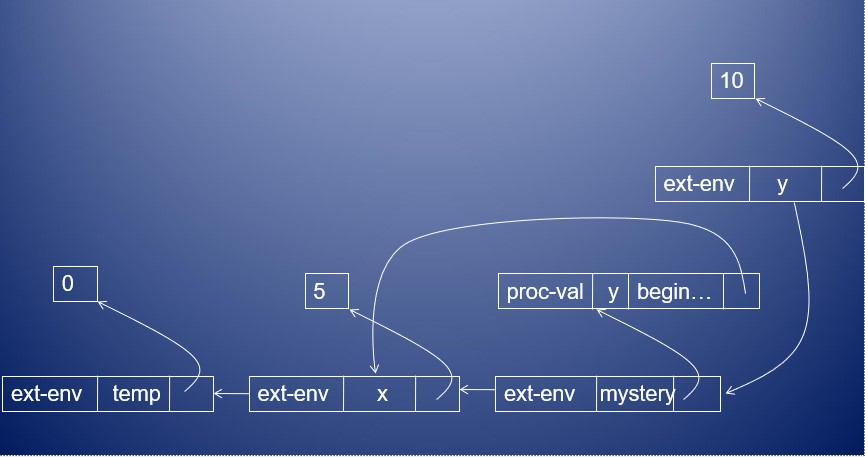
\includegraphics[scale=0.5]{mystery1.jpg}
\end{center}

\end{itemize}
\end{scriptsize}
\end{frame}

\begin{frame}[fragile]
\frametitle{Language with Explicit References}
%\framesubtitle{HOMEWORK}
\begin{scriptsize}
\begin{itemize}
\item<1->
\begin{alltt}
let temp = newref(0)
in  let x = newref(5)
    in  let mystery = proc (y)
                        begin
                          \textcolor{red}{setref(temp, deref(x)));}
                          setref(x, deref(y));
                          setref(y, deref(temp));
                          deref(x)
				        end
	    in (mystery newref(10))
\end{alltt}

\item<1->
\begin{center}
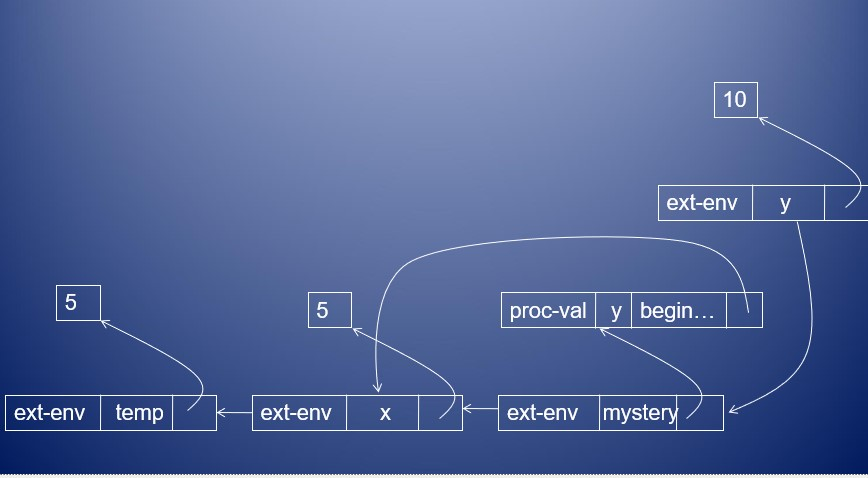
\includegraphics[scale=0.5]{mystery2.jpg}
\end{center}

\end{itemize}
\end{scriptsize}
\end{frame}

\begin{frame}[fragile]
\frametitle{Language with Explicit References}
%\framesubtitle{HOMEWORK}
\begin{scriptsize}
\begin{itemize}
\item<1->
\begin{alltt}
let temp = newref(0)
in  let x = newref(5)
    in  let mystery = proc (y)
                        begin
                          setref(temp, deref(x)));
                          \textcolor{red}{setref(x, deref(y));}
                          setref(y, deref(temp));
                          deref(x)
				        end
	    in (mystery newref(10))
\end{alltt}

\item<1->
\begin{center}
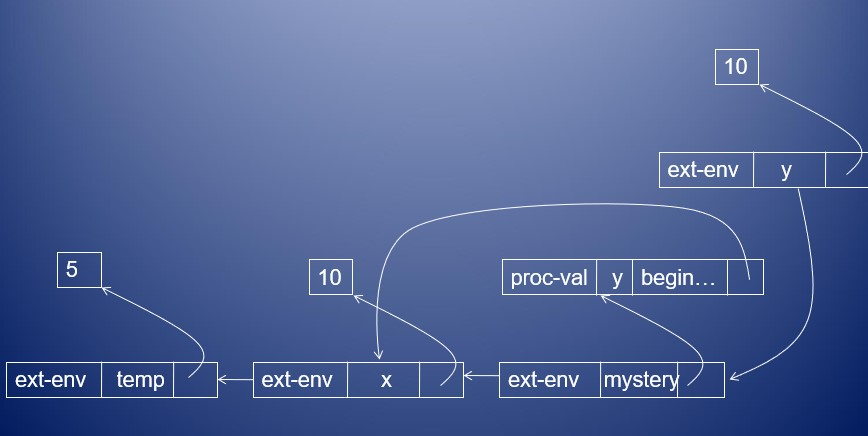
\includegraphics[scale=0.5]{mystery3.jpg}
\end{center}

\end{itemize}
\end{scriptsize}
\end{frame}

\begin{frame}[fragile]
\frametitle{Language with Explicit References}
%\framesubtitle{HOMEWORK}
\begin{scriptsize}
\begin{itemize}
\item<1->
\begin{alltt}
let temp = newref(0)
in  let x = newref(5)
    in  let mystery = proc (y)
                        begin
                          setref(temp, deref(x)));
                          setref(x, deref(y));
                          \textcolor{red}{setref(y, deref(temp));}
                          deref(x)
				        end
	    in (mystery newref(10))
\end{alltt}

\item<1->
\begin{center}
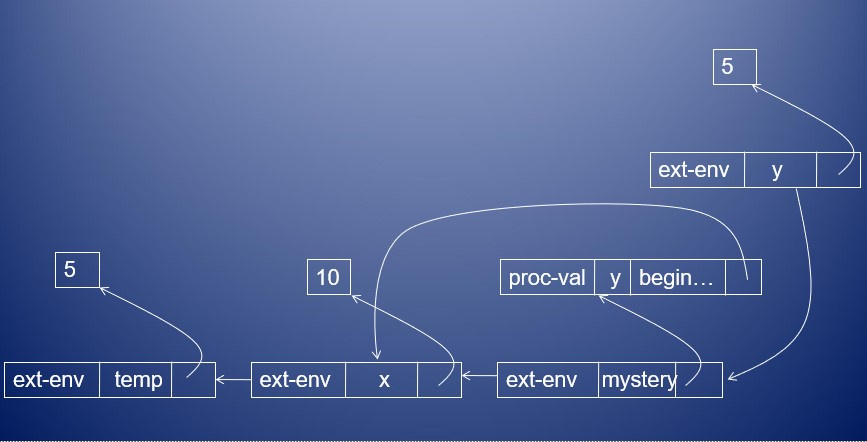
\includegraphics[scale=0.5]{mystery4.jpg}
\end{center}

\item<1-> Returns: 10

\end{itemize}
\end{scriptsize}
\end{frame}

\begin{frame}[fragile]
\frametitle{Language with Explicit References}
%\framesubtitle{HOMEWORK}
\begin{scriptsize}
\begin{itemize}
\item<1-> Is this a valid program? If so, what does it evaluate to?
\begin{alltt}
let x = newref(newref(10))
in begin
	setref(deref(x), 20));
	 +(20, deref(deref(x)))
   end
\end{alltt}

\end{itemize}
\end{scriptsize}
\end{frame}

\begin{frame}[fragile]
\frametitle{Language with Explicit References}
%\framesubtitle{HOMEWORK}
\begin{scriptsize}
\begin{itemize}
\item<1->
\begin{alltt}
let x = newref(\textcolor{red}{newref(10)})
in begin
	setref(deref(x), 20));
	 +(20, deref(deref(x)))
   end
\end{alltt}

\item<1->
\begin{center}

\includegraphics[scale=0.5]{pointer-chain1.jpg}
\end{center}

\end{itemize}
\end{scriptsize}
\end{frame}

\begin{frame}[fragile]
\frametitle{Language with Explicit References}
%\framesubtitle{HOMEWORK}
\begin{scriptsize}
\begin{itemize}
\item<1-> Is this a valid program? If so, what does it evaluate to?
\begin{alltt}
let x = \textcolor{red}{newref(}newref(10)\textcolor{red}{)}
in begin
	setref(deref(x), 20));
	 +(20, deref(deref(x)))
   end
\end{alltt}

\item<1->
\begin{center}

\includegraphics[scale=0.5]{pointer-chain2.jpg}
\end{center}

\end{itemize}
\end{scriptsize}
\end{frame}

\begin{frame}[fragile]
\frametitle{Language with Explicit References}
%\framesubtitle{HOMEWORK}
\begin{scriptsize}
\begin{itemize}
\item<1-> Is this a valid program? If so, what does it evaluate to?
\begin{alltt}
\textcolor{red}{let x =} newref(newref(10))
in begin
	setref(deref(x), 20));
	 +(20, deref(deref(x)))
   end
\end{alltt}

\item<1->
\begin{center}
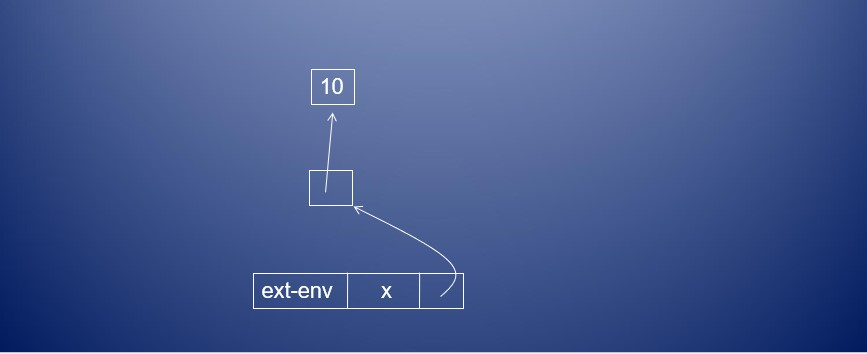
\includegraphics[scale=0.5]{pointer-chain3.jpg}
\end{center}

\end{itemize}
\end{scriptsize}
\end{frame}

\begin{frame}[fragile]
\frametitle{Language with Explicit References}
%\framesubtitle{HOMEWORK}
\begin{scriptsize}
\begin{itemize}
\item<1-> Is this a valid program? If so, what does it evaluate to?
\begin{alltt}
let x = newref(newref(10))
in begin
	\textcolor{red}{setref(deref(x), 20));}
	+(20, deref(deref(x)))
   end
\end{alltt}

\item<1->
\begin{center}
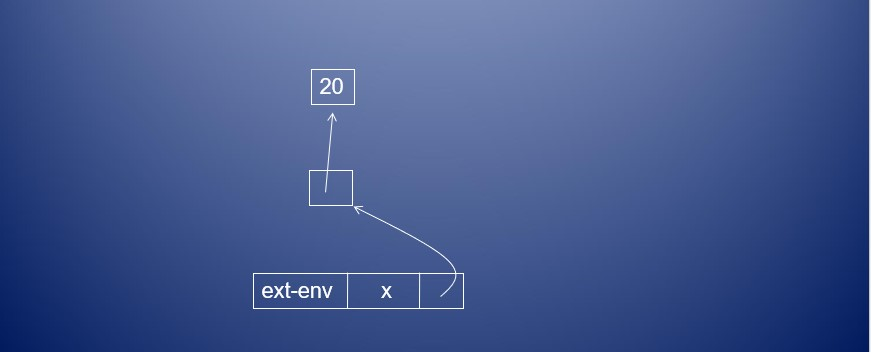
\includegraphics[scale=0.5]{pointer-chain4.jpg}
\end{center}

\end{itemize}
\end{scriptsize}
\end{frame}

\begin{frame}[fragile]
\frametitle{Language with Explicit References}
%\framesubtitle{HOMEWORK}
\begin{scriptsize}
\begin{itemize}
\item<1-> Is this a valid program? If so, what does it evaluate to?
\begin{alltt}
let x = newref(newref(10))
in begin
	setref(deref(x), 20));
	\textcolor{red}{+(20, deref(deref(x)))}
   end
\end{alltt}

\item<1->
\begin{center}
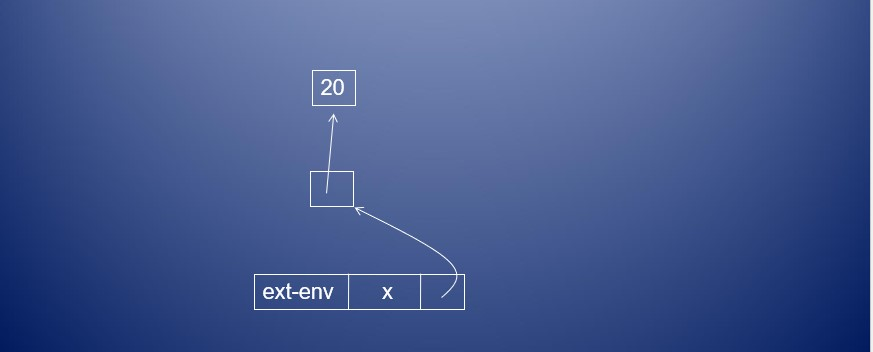
\includegraphics[scale=0.5]{pointer-chain5.jpg}
\end{center}

\item<1-> Returns 40
\end{itemize}
\end{scriptsize}
\end{frame}

\begin{frame}[fragile]
\frametitle{Language with Explicit References}
%\framesubtitle{HOMEWORK}
\begin{scriptsize}
\begin{itemize}
\item<1-> Expressed Values
\begin{alltt}
(define-datatype expval expval?
  (num-val
   (value number?))
  (bool-val
   (boolean boolean?))
  (proc-val
   (proc proc?))
  \textcolor{red}{(ref-val
   (ref reference?))})
\end{alltt}

\item<2->
\begin{alltt}
;; expval --> ref throws error
;; Purpose: Extract ref from given expval
(define (expval2ref v)
  (cases expval v
    (ref-val (ref) ref)
    (else (expval-extractor-error \quot{}reference v))))
\end{alltt}

\end{itemize}
\end{scriptsize}
\end{frame}

\begin{frame}[fragile]
\frametitle{Language with Explicit References}
%\framesubtitle{HOMEWORK}
\begin{scriptsize}
\begin{itemize}
\item<1-> To have \emph{effects} values must be stored somewhere

\item<2-> $\sigma$ ranges over the store (or heap)

\item<2-> $\left[l = v\right]$$\sigma$  \arrow{} the store $\sigma$ extended with location l mapped to v

\item<3-> We shall think of the store as an argument to value-of

\item<3-> (value-of exp1 $\rho$ $\sigma_0$) = (val1, $\sigma_1$)

\item<3-> $\sigma_0$ may or may not be the same as $\sigma_1$

\end{itemize}
\end{scriptsize}
\end{frame}

\begin{frame}[fragile]
\frametitle{Language with Explicit References}
\framesubtitle{Specification}
\begin{normalsize}
\begin{itemize}
\item<1-> (value-of (const-exp n) $\rho$ $\sigma$) = ((numval n), $\sigma$)

\item<2-> $\frac{(value\text{-}of \ exp1 \ \rho \ \sigma_0) \ = \ (val1, \ \sigma_1) \ \wedge \ (value\text{-}of \ exp2 \ \rho \ \sigma_1) \ = \ (val2, \ \sigma_2)}{(value\text{-}of \ (diff\text{-}exp \ exp1 \ exp2) \ \rho \ \sigma_0) \ = \ ((num\text{-}val \ val1 - val2) \ \sigma_2)}$

\item<3->
\begin{scriptsize}
$\frac{(value\text{-}of e1 \ \rho \ \sigma_0) \ = \ (v1, \sigma_1)
}{(value\text{-}of (if\text{-}exp \ e1 \ e2 \ e3) \ \rho \ \sigma_0) = \begin{cases}
       ((value\text{-}of \ e2 \ \rho \ \sigma_1), \sigma_2) & \text{if (exp\arrow{}val v1) = \#t
} \\
       ((value\text{-}of \ e3 \ \rho \ \sigma_1), \sigma_2) & \text{otherwise}
  \end{cases}}$
\end{scriptsize}

\end{itemize}
\end{normalsize}
\end{frame}

\begin{frame}[fragile]
\frametitle{Language with Explicit References}
\framesubtitle{Specification}
\begin{scriptsize}
\begin{itemize}
\item<1-> $\frac{(value\text{-}of \ exp \ \rho \ \sigma_0) \ = \ (val1, \ \sigma_1)	\ l\notin dom(\sigma_0)
}{(value\text{-}of \ (newref\text{-}exp \ exp) \ \rho \ \sigma_0) =   ((ref\text{-}val \ l), \ \left[l =  val1\right]\sigma_1)}$

\item<1-> l is a new store location

\item<2-> $\frac{(value\text{-}of exp \ \rho \ \sigma_0) \ = \ (l, \ \sigma_1)}{(value\text{-}of \ (deref\text{-}exp \ exp) \ \rho \ \sigma_0) \ =  \ (\sigma_1(l), \ \sigma_1)}$

\item<3-> $\frac{(value\text{-}of \ exp1 \ \rho \ \sigma_0) \ = \ (l, \ \sigma_1) \ \wedge \ (value\text{-}of \ exp2 \ \rho \ \sigma_1) = (val, \ \sigma_2)}{(value\text{-}of (setref\text{-}exp \ exp1 \ exp2) \ \rho \ \sigma_0) \ = \ (\varnothing, \ \left[ l =  val\right] \sigma_2)}$

\end{itemize}
\end{scriptsize}
\end{frame}

\begin{frame}[fragile]
\frametitle{Language with Explicit References}
\framesubtitle{Implementation}
\begin{scriptsize}
\begin{itemize}
\item<1-> Grammar
\begin{alltt}
(expression ("begin" expression (arbno ";" expression) "end")
            begin-exp)

(expression ("newref" "(" expression ")") newref-exp)

(expression ("deref" "(" expression ")") deref-exp)

(expression ("setref" "(" expression "," expression ")")
            setref-exp)
\end{alltt}

\end{itemize}
\end{scriptsize}
\end{frame}

\begin{frame}[fragile]
\frametitle{Language with Explicit References}
\framesubtitle{Implementation}
\begin{scriptsize}
\begin{itemize}
\item<1-> Design choice: the store is a global variable

\item<1-> Design choice: Represent the store as a (listof expval)

\item<2->
\begin{alltt}
;; reference? : RacketVal --> Bool
(define (reference? v) (and (integer? v) (>= v 0)))
\end{alltt}

\item<3->
\begin{alltt}
;; the-store: the current state of the  store
(define the-store \quot{}uninitialized)
\end{alltt}

\item<4->
\begin{alltt}
;; empty-store :  --> store
(define (empty-store) \elist{})
\end{alltt}

\item<5->
\begin{alltt}
;; initialize-store! :  --> store
(define (initialize-store!) (set! the-store (empty-store)))
\end{alltt}

\item<6->
\begin{alltt}
;; newref : expval --> ref
(define (newref val)
  (let ((next-ref (length the-store)))
    (set! the-store (append the-store (list val)))
    next-ref))
\end{alltt}

\item<7->
\begin{alltt}
;; deref : ref --> expval
(define (deref ref) (list-ref the-store ref))
\end{alltt}

\item<8->
\begin{alltt}
;; setref : ref expval --> expval
(define (setref! ref new-expval)
  (set! the-store (append (take the-store ref)
                          (list new-expval)
                          (drop the-store (add1 ref)))))
\end{alltt}

\end{itemize}
\end{scriptsize}
\end{frame}

\begin{frame}[fragile]
\frametitle{Language with Explicit References}
\framesubtitle{Implementation}
\begin{scriptsize}
\begin{itemize}
\item<1->
\begin{alltt}
;; value-of-program : program --> expval
(define (value-of-program pgm)
  (begin
    (initialize-store!)
    (cases program pgm
      (a-program (exp1)
                 (value-of exp1 (empty-env))))))
\end{alltt}

\end{itemize}
\end{scriptsize}
\end{frame}

\begin{frame}[fragile]
\frametitle{Language with Explicit References}
\framesubtitle{Implementation}
\begin{tiny}
\begin{itemize}
\item<1->
\begin{alltt}
(define (value-of exp env)
  (cases expression exp
    (const-exp (num) (num-val num))
    (true-exp () (bool-val #t))
    (false-exp () (bool-val #f))
\end{alltt}

\item<2->
\begin{alltt}
    (var-exp (var) (apply-env env var))
\end{alltt}

\item<3->
\begin{alltt}
    (diff-exp (exp1 exp2)
              (let ((num1 (expval2num (value-of exp1 env)))
                    (num2 (expval2num (value-of exp2 env))))
                (num-val (- num1 num2))))
\end{alltt}

\item<4->
\begin{alltt}
    (zero?-exp (exp1)
               (let ((val1 (expval2num (value-of exp1 env))))
                 (if (zero? val1)
                     (bool-val #t)
                     (bool-val #f))))
\end{alltt}

\item<5->
\begin{alltt}
    (if-exp (exp1 exp2 exp3)
            (let ((val1 (value-of exp1 env)))
              (if (expval2bool val1)
                  (value-of exp2 env)
                  (value-of exp3 env))))
\end{alltt}

\item<6->
\begin{alltt}
    (let-exp (vars exps body)
             (let [(vals (map (lambda (e) (value-of e env)) exps))]
               (value-of body
                         (foldr (lambda (var val acc)
                                  (extend-env var val acc))
                                env
                                vars
                                vals))))
    \vdotss
\end{alltt}

\end{itemize}
\end{tiny}
\end{frame}

\begin{frame}[fragile]
\frametitle{Language with Explicit References}
\framesubtitle{Implementation}
\begin{tiny}
\begin{itemize}
\item<1->
\begin{alltt}
(define (value-of exp env)
  (cases expression exp
    \vdotss{}
    (proc-exp (params body)
              (proc-val (procedure params body (vector env))))
\end{alltt}

\item<2->
\begin{alltt}
    (call-exp (rator rands)
              (let [(proc (expval2proc (value-of rator env)))
                    (args (map (lambda (rand) (value-of rand env)) rands))]
                (apply-procedure proc args)))
\end{alltt}

\item<3->
\begin{alltt}
    (letrec-exp (names params bodies letrec-body)
                (value-of letrec-body (mk-letrec-env names params bodies env)))
\end{alltt}

\item<4->
\begin{alltt}
    (begin-exp (exp exps)
               (foldl (lambda (e v) (value-of e env)) (value-of exp env) exps))
\end{alltt}

\item<5->
\begin{alltt}
    (newref-exp (exp1)
                (let ((v1 (value-of exp1 env)))
                  (ref-val (newref v1))))
\end{alltt}

\item<6->
\begin{alltt}
    (deref-exp (exp1)
               (let ((v1 (value-of exp1 env)))
                 (let ((ref1 (expval2ref v1)))
                   (deref ref1))))
\end{alltt}

\item<7->
\begin{alltt}
    (setref-exp (exp1 exp2)
                (let ((ref (expval2ref (value-of exp1 env))))
                  (let ((v2 (value-of exp2 env)))
                    (begin
                      (setref! ref v2)
                      (num-val -1)))))))
\end{alltt}

\end{itemize}
\end{tiny}
\end{frame}

\begin{frame}[fragile]
\frametitle{Language with Explicit References}
\framesubtitle{Homework}
\begin{scriptsize}
\begin{itemize}
\item<1-> 4.1, 4.2, 4.4, 4.8, 4.9

\end{itemize}
\end{scriptsize}
\end{frame}


\section{Language with Implicit References}

\begin{frame}[fragile]
\frametitle{Language with Implicit References}
%\framesubtitle{HOMEWORK}
\begin{scriptsize}
\begin{itemize}
\item<1-> Most modern PLs package common patterns of allocation, dereferencing, and mutation

\item<1-> Programmers do not need to worry about these operations

\item<2-> Every variable denotes a reference
\item<2-> References are no longer expressed values and exist only as bindings of vars
\begin{alltt}
		expval = int + bool + proc
		denval = ref(expval)
\end{alltt}

\item<3-> Locations are created with each binding operation: procedure call, let, and letrec

\item<4-> What happens when the interpreter encounters a var-exp?
\begin{itemize}
\item env look-up to find the location to which it’s bound
\item look-up in the store to find the value at that location
\item two-level system for var-exps
\end{itemize}

\end{itemize}
\end{scriptsize}
\end{frame}

\begin{frame}[fragile]
\frametitle{State}
%\framesubtitle{HOMEWORK}
\begin{scriptsize}
\begin{itemize}
\item<1-> The content of a location can be changed (or mutated)
	
\item<1-> expression \arrow{} set identifier = expression

\item<1-> the identifier is \emph{not} an expression; not evaluated

\item<1-> vars are mutable

\item<2-> Extend LETREC language and implement call-by-value semantics

\item<2-> \emph{Values} are passed to every function

\item<2-> Formal parameters bound to locations of operand values

\item<2-> It is the most common form of parameter passing

\item<3-> Why are chains of references not possible?

\item<4-> Refs are not expressed values

\end{itemize}
\end{scriptsize}
\end{frame}

\begin{frame}[fragile]
\frametitle{State}
%\framesubtitle{HOMEWORK}
\begin{scriptsize}
\begin{itemize}
\item<1-> Consider
\begin{alltt}
\textcolor{red}{let a = 3}
in let p = proc (x) set x = 4
   in begin (p a); a end
\end{alltt}

\item<2->
\begin{center}
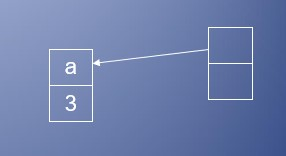
\includegraphics[scale=0.5]{cbv1.jpg}
\end{center}

\end{itemize}
\end{scriptsize}
\end{frame}

\begin{frame}[fragile]
\frametitle{State}
%\framesubtitle{HOMEWORK}
\begin{scriptsize}
\begin{itemize}
\item<1-> Consider
\begin{alltt}
let a = 3
in \textcolor{red}{let p = proc (x) set x = 4}
   in begin (p a); a end
\end{alltt}

\item<1->
\begin{center}
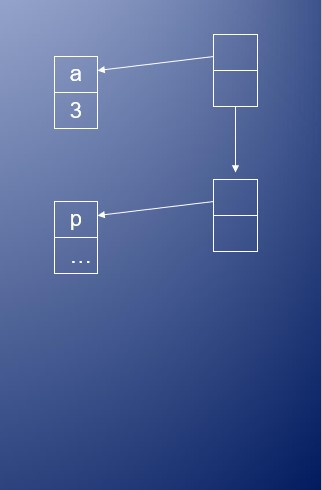
\includegraphics[scale=0.5]{cbv2.jpg}
\end{center}

\end{itemize}
\end{scriptsize}
\end{frame}

\begin{frame}[fragile]
\frametitle{State}
%\framesubtitle{HOMEWORK}
\begin{scriptsize}
\begin{itemize}
\item<1-> Consider
\begin{alltt}
let a = 3
in let p = proc (x) set x = 4
   in begin \textcolor{red}{(p a);} a end
\end{alltt}

\item<1->
\begin{center}
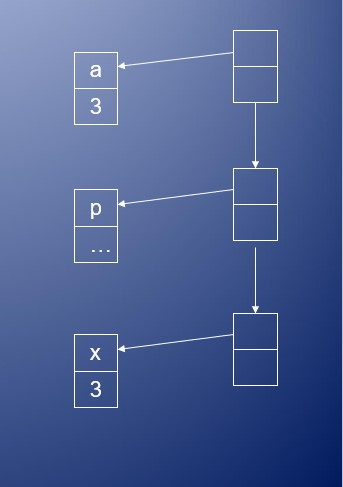
\includegraphics[scale=0.5]{cbv3.jpg}
\end{center}

\end{itemize}
\end{scriptsize}
\end{frame}

\begin{frame}[fragile]
\frametitle{State}
%\framesubtitle{HOMEWORK}
\begin{scriptsize}
\begin{itemize}
\item<1-> Consider
\begin{alltt}
let a = 3
in let p = proc (x) \textcolor{red}{set x = 4}
   in begin (p a); a end
\end{alltt}

\item<1->
\begin{center}
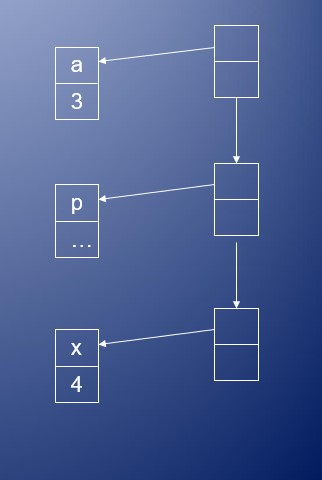
\includegraphics[scale=0.5]{cbv4.jpg}
\end{center}

\item<1-> Returns 3

\end{itemize}
\end{scriptsize}
\end{frame}

\begin{frame}[fragile]
\frametitle{State}
\framesubtitle{Specification}
\begin{scriptsize}
\begin{itemize}
\item<1-> $(value\text{-}of (var\text{-}exp v) \ \rho \ \sigma) \ = \ (\sigma(\rho(v)), \ \sigma)$

\item<1-> Get v's binding (a reference) and access store for v's expval

\item<1-> The store is unchanged\newline

\item<2-> $\frac{(value\text{-}of \ exp1 \ \rho \ \sigma_0) \ = \ (val1, \ \sigma_1)
}{(value\text{-}of (set\text{-}exp \ v \ exp1) \ \rho \ \sigma_0) \ = \ (\varnothing, \ \left[\sigma{}(v) = val1\right] \sigma_1)}$

\item<2-> The location of v is changed to store val1

\item<2-> The original value stored in $\sigma$(v) is lost forever \newline

\item<3-> $(apply\text{-}procedure \ (procedure \ v \ b \ \rho) \ val \ \sigma) \newline = \ (value\text{-}of \ b \ [v = l]\rho \ [l = val]\sigma)$

\item<3-> The body is evaluated in a store where l contains the value of the parameter and an environment that binds the parameter to l

\item<4-> $\frac{(value\text{-}of \ exp1 \ \rho \ \sigma)  = (val, \ \sigma_1)}{(value\text{-}of \ (let\text{-}exp \ var \ exp1 \ exp2) \ \rho \ \sigma) = (value\text{-}of \ exp2 \ [var = l]\rho \ \left[l = val\right]\sigma_1)}$

\item<4-> Evaluate the body of the let-exp in a store where l contains the value of the local variable and the local variable is bound to l

\end{itemize}
\end{scriptsize}
\end{frame}

\begin{frame}[fragile]
\frametitle{State}
%\framesubtitle{HOMEWORK}
\begin{scriptsize}
\begin{itemize}
\item<1-> $\frac{(value\text{-}of \ e0 \ \rho \ \sigma_0)=(p, \ \sigma_1) \ \wedge \ (value\text{-}of \ e1 \ \rho \ \sigma_1)=(v1, \sigma_2) \ \wedge \ (value\text{-}of \ e2 \ \rho \ \sigma_2)=(v2, \ \sigma_3) \wedge \ \ldots}
    {(value\text{-}of \ (call\text{-}exp \ e0 \ e1\ldots en) \ \rho \ \sigma_0) = (apply\text{-}procedure \ p \ v1\ldots vn \ \sigma_{n+1})}$

\item<1-> Evaluate all expressions using the given environment

\item<1-> Evaluate $ei$ using $\sigma_i$

\item<1-> Apply the proc to the args using the store state after evaluating all expressions \newline

\item<2-> $\frac{\rho_n=\left[n_1=l_1\ldots n_n=l_n\right]\rho \ \wedge \ p1=(proc\text{-}val \ n_1 \ p_1 \ e_1 \ \rho_n) \ \wedge \ldots \wedge \ pn=(proc\text{-}val \ n_n \ p_n \ e_n \ \rho_n)}
                {(v\text{-}o \ (letrec\text{-}exp \ n_1\ldots n_n \ p_1\ldots p_n \ e_1\dots e_n \ e_{n+1}) \ \rho \ \sigma)=(v\text{-}o \ e_{n+1} \ \rho_n \ \left[l_1=p1\ldots l_n=pn \right]\sigma)}$

\item<2-> v-o = value-of

\item<2-> All procs are allocated in the store

\end{itemize}
\end{scriptsize}
\end{frame}

\begin{frame}[fragile]
\frametitle{State}
\framesubtitle{Implementation}
\begin{scriptsize}
\begin{itemize}
\item<1->
\begin{alltt}
(expression
     ("begin" expression (arbno ";" expression) "end")
     begin-exp)

(expression ("set" identifier "=" expression)  set-exp)
\end{alltt}

\item<2-> The store is the same as with Explicit Refs

\item<3->
\begin{alltt}
(define-datatype expval expval?
  (num-val
   (value number?))
  (bool-val
   (boolean boolean?))
  (proc-val
   (proc proc?)))
\end{alltt}

\item<3-> Unlike Explicit Refs, no ref-val

\item<4-> Same as Explicit Refs
\begin{alltt}
(define (value-of-program pgm)
  (begin
    (initialize-store!)
    (cases program pgm
      (a-program (exp1)
                 (value-of exp1 (empty-env))))))
\end{alltt}

\end{itemize}
\end{scriptsize}
\end{frame}

\begin{frame}[fragile]
\frametitle{State}
\framesubtitle{Implementation}
\begin{scriptsize}
\begin{itemize}
\item<1->
\begin{alltt}
(check-equal? (eval "if zero?(1) then 1 else 2")
              (num-val 2))

(check-equal? (eval "-(15, 10)")
              (num-val 5))

(check-equal?
  (eval "let x = 10 in if zero?(-(x, x)) then x else 2")
  (num-val 10))

(check-equal? (eval "let decr = proc (a) -(a, 1) in (decr 30)")
              (num-val 29))

(check-equal? (eval "( proc (g) (g 30) proc (y) -(y, 1))")
              (num-val 29))

(check-equal? (eval "let x = 200
                     in let f = proc (z) -(z, x)
                        in let x = 100
                           in let g = proc (z) -(z, x)
                              in -((f 1), (g 1))")
              (num-val -100))
\end{alltt}

\end{itemize}
\end{scriptsize}
\end{frame}

\begin{frame}[fragile]
\frametitle{State}
\framesubtitle{Implementation}
\begin{scriptsize}
\begin{itemize}
\item<1->
\begin{alltt}
(check-equal?
  (eval "let sum = proc (x) proc (y) -(x, -(0, y)) in ((sum 3) 4)")
  (num-val 7))

(check-equal?
  (eval "let sum = proc (x) proc (y) -(x, -(0, y))
         in letrec sigma (n) = if zero?(n)
                               then 0
                               else ((sum n) (sigma -(n, 1)))
            in (sigma 5)")
  (num-val 15))

(check-equal? (eval "letrec even(n) = if zero?(n)
                                      then zero?(n)
                                      else if zero?(-(n, 1))
                                           then zero?(n)
                                           else (even -(n, 2))
                     in (even 501)")
              (bool-val \#f))
\end{alltt}

\end{itemize}
\end{scriptsize}
\end{frame}

\begin{frame}[fragile]
\frametitle{State}
\framesubtitle{Implementation}
\begin{scriptsize}
\begin{itemize}
\item<1->
\begin{alltt}
\textcolor{red}{(check-equal? (eval "let a = 3
                     in let p = proc (x) set x = 4
                        in begin
                             (p a);
                             a
                           end")
              (num-val 3))}

\textcolor{red}{(check-equal? (eval "let x = 0
                     in letrec f (x) = set x = +(x, 1)
                               g (a) = set x = +(x, 2)
                        in begin
                             (f x);
                             (g x);
                             x
                           end")
              (num-val 2))}
\end{alltt}

\end{itemize}
\end{scriptsize}
\end{frame}

\begin{frame}[fragile]
\frametitle{State}
\framesubtitle{Implementation}
\begin{scriptsize}
\begin{itemize}
\item<1->
\begin{alltt}
(define (value-of exp env)
  (cases expression exp

    (const-exp (num) (num-val num))

    (true-exp () (bool-val #t))

    (false-exp () (bool-val #f))

    (var-exp (var) (deref (apply-env env var)))

    (diff-exp (exp1 exp2)
              (let ((num1 (expval2num (value-of exp1 env)))
                    (num2 (expval2num (value-of exp2 env))))
                (num-val (- num1 num2))))

    (zero?-exp (exp1)
               (let ((val1 (expval2num (value-of exp1 env))))
                 (if (zero? val1)
                     (bool-val #t)
                     (bool-val #f))))
\end{alltt}

\end{itemize}
\end{scriptsize}
\end{frame}

\begin{frame}[fragile]
\frametitle{State}
\framesubtitle{Implementation}
\begin{scriptsize}
\begin{itemize}
\item<1->
\begin{alltt}
    (if-exp (exp1 exp2 exp3)
        (let ((val1 (value-of exp1 env)))
          (if (expval2bool val1)
              (value-of exp2 env)
              (value-of exp3 env))))

    (let-exp (vars exps body)
             (let [(vals (map (lambda (e) (value-of e env)) exps))]
              (value-of body
                        (foldr (lambda (var val acc)
                                (extend-env var \textcolor{red}{(newref val)} acc))
                               env
                               vars
                               vals))))

    (proc-exp (params body)
              (proc-val (procedure params body (vector env))))

    (call-exp (rator rands)
              (let [(proc (expval2proc (value-of rator env)))
                    (args (map (lambda (rand) (value-of rand env)) rands))]
                (apply-procedure proc args)))
\end{alltt}

\end{itemize}
\end{scriptsize}
\end{frame}

\begin{frame}[fragile]
\frametitle{State}
\framesubtitle{Implementation}
\begin{scriptsize}
\begin{itemize}
\item<1->
\begin{alltt}
    (letrec-exp (names params bodies rec-body)
      (value-of rec-body (mk-letrec-env names params bodies env)))

    (begin-exp (exp exps)
      (foldl (lambda (e v) (value-of e env))
             (value-of exp env)
             exps))

    \textcolor{red}{(set-exp (var exp1)
             (begin
               (setref! (apply-env env var) (value-of exp1 env))
               (num-val 31)))}))
\end{alltt}

\end{itemize}
\end{scriptsize}
\end{frame}

\begin{frame}[fragile]
\frametitle{State}
\framesubtitle{Implementation}
\begin{scriptsize}
\begin{itemize}
\item<1->
\begin{alltt}
(define (mk-letrec-env names params bodies env)
  (let* [(temp-proc-vals
           (map (lambda (p b)
                  (proc-val (procedure p b (vector (empty-env)))))
                params
                bodies))
         (new-env (foldl (lambda (name proc env)
                           (extend-env name
                                       \textcolor{red}{(newref proc)}
                                       env))
                         env
                         names
                         temp-proc-vals))]
    (begin
      (for-each (lambda (p)
                  (cases proc p
                    (procedure (p b ve)
                               (vector-set! ve 0 new-env))))
                (map (lambda (p) (expval2proc p))
                     temp-proc-vals))
      new-env)))
\end{alltt}

\end{itemize}
\end{scriptsize}
\end{frame}

\begin{frame}[fragile]
\frametitle{State}
\framesubtitle{Implementation}
\begin{scriptsize}
\begin{itemize}
\item<1->
\begin{alltt}
(define (apply-procedure f vals)
  (cases proc f
    (procedure (params body envv)
      (let [(saved-env (vector-ref envv 0))]
        (value-of body
                  (foldr (lambda (binding acc)
                           (extend-env (car binding)
                                       \textcolor{red}{(newref (cadr binding))}
                                       acc))
                         saved-env
                         (map (lambda (p v) (list p v))
                              params
                              vals)))))))
\end{alltt}

\end{itemize}
\end{scriptsize}
\end{frame}


\section{Mutable Pairs}

\begin{frame}[fragile]
%\frametitle{Definition and Implementation}
%\framesubtitle{HOMEWORK}
\begin{scriptsize}
\begin{itemize}
\item<1-> We will add mutable pairs to IMPLICIT-REFS

\item<2-> expval = int + bool + proc + mutpair

\item<2-> mutpair = ref(expval) x ref(expval)
		
\item<3-> DenVal = ref(expval)

\item<4-> Specification
\begin{itemize}
\item[\arrow] newpair: expval  expval \arrow{} mutpair
\item[\arrow] left: mutpair \arrow{} expval
\item[\arrow] right: mutpair \arrow{} expval
\item[\arrow] setleft: mutpair expval \arrow{} $\varnothing$
\item[\arrow] setright: mutpair expval \arrow{} $\varnothing$
\end{itemize}

		
\item<5->
\begin{alltt}
(define-datatype expval expval?
  (num-val
   (value number?))
  (bool-val
   (boolean boolean?))
  (proc-val
   (proc proc?))
  \textcolor{red}{(mutpair-val} ;; new for mutable pairs
   \textcolor{red}{(p mutpair?))})
\end{alltt}

\end{itemize}
\end{scriptsize}
\end{frame}

\begin{frame}[fragile]
%\frametitle{Definition and Implementation}
%\framesubtitle{HOMEWORK}
\begin{scriptsize}
\begin{itemize}
\item<1-> Grammar
\begin{itemize}
\item[\arrow] (expression ("newpair" "(" expression "," expression ")") newpair-exp)

\item[\arrow] (expression ("left" "(" expression ")") left-exp)

\item[\arrow] (expression ("setleft" expression "=" expression) setleft-exp)

\item[\arrow] (expression ("right" "(" expression ")") right-exp)

\item[\arrow] (expression ("setright" expression "=" expression) setright-exp)
\end{itemize}

\end{itemize}
\end{scriptsize}
\end{frame}

\begin{frame}[fragile]
%\frametitle{Definition and Implementation}
%\framesubtitle{HOMEWORK}
\begin{scriptsize}
\begin{itemize}
\item<1-> Let's trace
\begin{alltt}
(eval "let \textcolor{red}{p = newpair(4, 5)}
       in begin
            setleft p = 15;
           	setright p = 15;
           	-(left(p), right(p))
          end")
\end{alltt}

\item<2->
\begin{center}
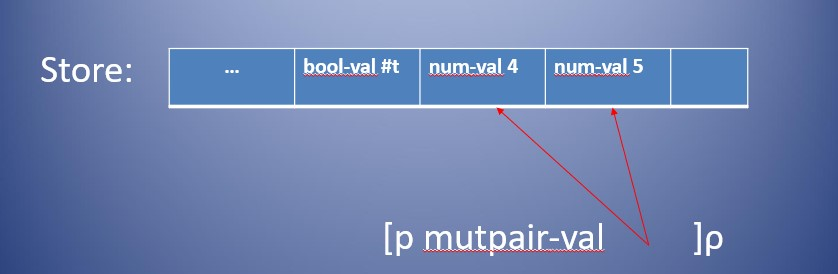
\includegraphics[scale=0.5]{mut-pairs1.jpg}
\end{center}

\end{itemize}
\end{scriptsize}
\end{frame}

\begin{frame}[fragile]
%\frametitle{Definition and Implementation}
%\framesubtitle{HOMEWORK}
\begin{scriptsize}
\begin{itemize}
\item<1-> Let's trace
\begin{alltt}
(eval "let p = newpair(4, 5)
       in begin
            \textcolor{red}{setleft p = 15;}
            setright p = 15;
            -(left(p), right(p))
          end")
\end{alltt}

\item<1->
\begin{center}
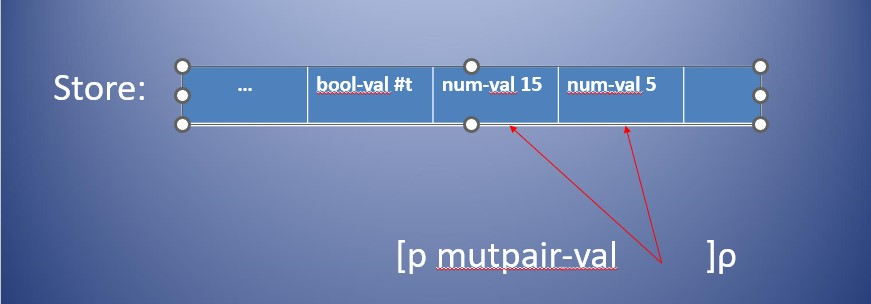
\includegraphics[scale=0.5]{mut-pairs2.jpg}
\end{center}

\end{itemize}
\end{scriptsize}
\end{frame}

\begin{frame}[fragile]
%\frametitle{Definition and Implementation}
%\framesubtitle{HOMEWORK}
\begin{scriptsize}
\begin{itemize}
\item<1-> Let's trace
\begin{alltt}
(eval "let p = newpair(4, 5)
       in begin
            setleft p = 15;
           	\textcolor{red}{setright p = 15;}
           	-(left(p), right(p))
          end")
\end{alltt}

\item<1->
\begin{center}
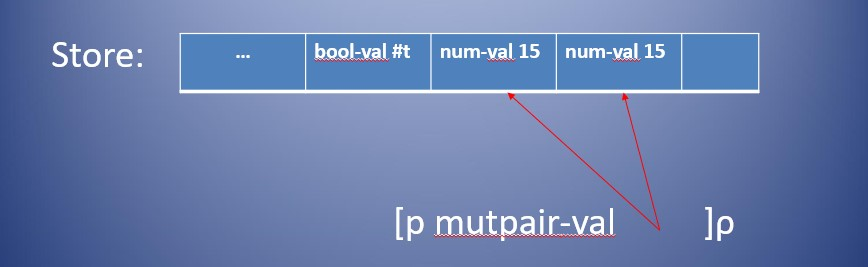
\includegraphics[scale=0.5]{mut-pairs3.jpg}
\end{center}

\item<1-> Returns (num-val 0)

\end{itemize}
\end{scriptsize}
\end{frame}

\begin{frame}[fragile]
%\frametitle{Definition and Implementation}
%\framesubtitle{HOMEWORK}
\begin{scriptsize}
\begin{itemize}
\item<1-> How can we represent a mutable pair?

\item<2->
\begin{alltt}
(define-datatype mutpair mutpair?
  (a-pair (left-loc reference?)
          (right-loc reference?)))
\end{alltt}

\item<2-> Is this a good implementation choice?

\item<3-> Does not take into account everything we know about mutable pairs
\begin{itemize}
\item[\arrow] The two locations are independently assignable
\item[\arrow] Not independently allocated
\end{itemize}

\item<4-> Consider newpair(4, 5) and $\sigma$
\begin{alltt}
     \(\sigma\) = ( \dotss )
     \(\sigma\) = ( \dotss 4)	
     \(\sigma\) = ( \dotss 4 5)
\end{alltt}

\item<5-> If the left is in position p in $\sigma$ , where is the right?

\item<6-> What does this tell you?

\item<7-> We can implement mutable pairs using a single reference

\end{itemize}
\end{scriptsize}
\end{frame}

\begin{frame}[fragile]
%\frametitle{Definition and Implementation}
%\framesubtitle{HOMEWORK}
\begin{scriptsize}
\begin{itemize}
\item<1->
\begin{alltt}
;; expval --> reference throws error
(define (expval->mutpair v)
  (cases expval v
    (mutpair-val (ref) ref)
    (else (expval-extractor-error 'mutable-pair v))))
\end{alltt}

\item<2->
\begin{alltt}
;; mutpair? : X -> Boolean
(define (mutpair? v) (reference? v))
\end{alltt}

\item<3->
\begin{alltt}
;; make-pair : expval expval -> mutpair
(define (make-pair val1 val2)
  (let ((ref1 (newref val1)))
    (let ((ref2 (newref val2)))
      ref1)))
\end{alltt}

\item<4->
\begin{alltt}
;; left : mutpair -> expval
(define (left p) (deref p))

;; right : mutpair -> expval
(define (right p) (deref (+ 1 p)))
\end{alltt}

\item<5->
\begin{alltt}
;; setleft : mutpair expval -> Unspecified
(define (setleft p val) (setref! p val))

;; setright : mutpair expval -> Unspecified
(define (setright p val) (setref! (+ 1 p) val))
\end{alltt}

\end{itemize}
\end{scriptsize}
\end{frame}

\begin{frame}[fragile]
%\frametitle{Definition and Implementation}
%\framesubtitle{HOMEWORK}
\begin{scriptsize}
\begin{itemize}
\item<1->
\begin{alltt}
     (check-equal? (eval "let p = newpair(4, 5)
                          in left(p)")
                   (num-val 4))

     (check-equal? (eval "let p = newpair(4, 5)
                          in right(p)")
                   (num-val 5))

     (check-equal? (eval "let p = newpair(4, 5)
                          in begin
                               setleft p = 15;
                               setright p = 15;
                               -(left(p), right(p))
                             end")
                   (num-val 0))
\end{alltt}

\end{itemize}
\end{scriptsize}
\end{frame}

\begin{frame}[fragile]
%\frametitle{Definition and Implementation}
%\framesubtitle{HOMEWORK}
\begin{scriptsize}
\begin{itemize}
\item<1->
\begin{alltt}
(define (value-of exp env)
  (cases expression exp
       \vdotss{}
    (newpair-exp (exp1 exp2)
      (let ((v1 (value-of exp1 env))
            (v2 (value-of exp2 env)))
        (mutpair-val (make-pair v1 v2))))
\end{alltt}

\item<2->
\begin{alltt}
    (left-exp (exp1)
      (let ((v1 (value-of exp1 env)))
        (let ((p1 (expval->mutpair v1)))
          (left p1))))
    (right-exp (exp1)
      (let ((v1 (value-of exp1 env)))
        (let ((p1 (expval->mutpair v1)))
          (right p1))))
\end{alltt}

\item<3->
\begin{alltt}
    (setleft-exp (exp1 exp2)
      (let ((v1 (value-of exp1 env))
            (v2 (value-of exp2 env)))
        (let ((p (expval->mutpair v1)))
          (begin (setleft p v2)
                 (num-val 82))))) ;; this is a don't care value.
    (setright-exp (exp1 exp2)
      (let ((v1 (value-of exp1 env))
            (v2 (value-of exp2 env)))
        (let ((p (expval->mutpair v1)))
          (begin (setright p v2)
                 (num-val 83))))) ;; this is a don't care value.
\end{alltt}

\end{itemize}
\end{scriptsize}
\end{frame}

\begin{frame}[fragile]
%\frametitle{Definition and Implementation}
%\framesubtitle{HOMEWORK}
\begin{scriptsize}
\begin{itemize}
\item<1-> Homework: 4.28--4.30
\end{itemize}
\end{scriptsize}
\end{frame}



\section{Parameter Passing Variations}

\begin{frame}[fragile]
\frametitle{Parameter Passing Variations}
\framesubtitle{Call by Reference}
\begin{scriptsize}
\begin{itemize}
\item<1-> In call-by-value semantics the callee is isolated from the caller

\item<1-> Assignments by the callee to its parameters can not be seen by the caller

\item<2-> Sometimes it is desirable to pass in variables expecting the callee to make assigments to them

\item<2-> This can be done by passing references to the callee instead of actual values

\item<2-> This is known as \emph{call-by-reference}

\item<3-> If an operand is a variable, then a reference to the variable’s location is passed

\item<3-> The formal parameter is bound to this location

\item<4-> If the operand is some other type of expression, then the formal parameter is bound to a new location containing the value of the operand

\item<4-> Just like in call-by-value

\end{itemize}
\end{scriptsize}
\end{frame}

\begin{frame}[fragile]
\frametitle{Parameter Passing Variations}
\framesubtitle{Call by Reference}
\begin{scriptsize}
\begin{itemize}
\item<1->
\begin{alltt}
let \textcolor{red}{a = 3}
	p = proc (x) set x = 4
in begin
    (p a);
    a
   end
\end{alltt}

\item<1->
\begin{center}
  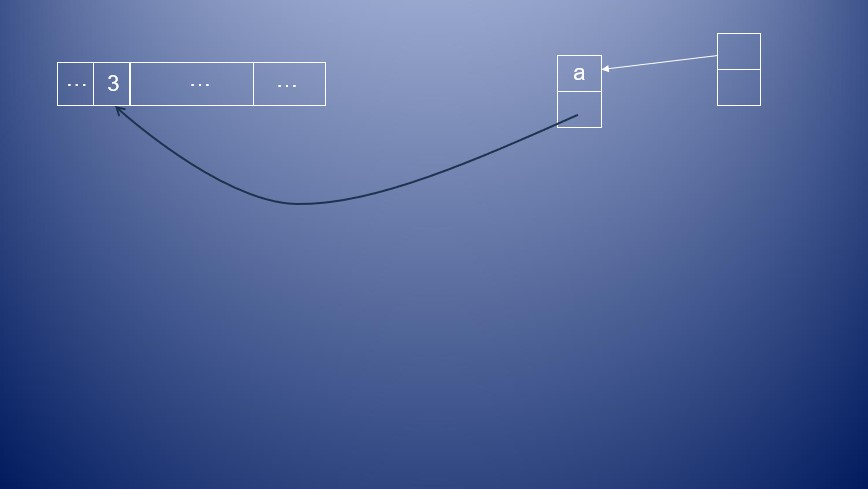
\includegraphics[scale=0.5]{cbr1.jpg}
\end{center}

\end{itemize}
\end{scriptsize}
\end{frame}

\begin{frame}[fragile]
\frametitle{Parameter Passing Variations}
\framesubtitle{Call by Reference}
\begin{scriptsize}
\begin{itemize}
\item<1->
\begin{alltt}
let a = 3
	\textcolor{red}{p = proc} (x) set x = 4
in begin
    (p a);
    a
   end
\end{alltt}

\item<1->
\begin{center}
  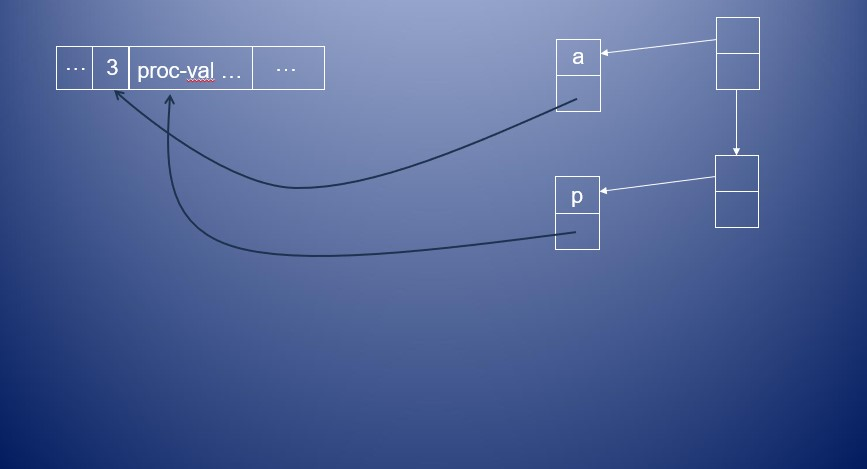
\includegraphics[scale=0.5]{cbr2.jpg}
\end{center}

\end{itemize}
\end{scriptsize}
\end{frame}

\begin{frame}[fragile]
\frametitle{Parameter Passing Variations}
\framesubtitle{Call by Reference}
\begin{scriptsize}
\begin{itemize}
\item<1->
\begin{alltt}
let a = 3
	p = proc (x) set x = 4
in begin
    \textcolor{red}{(p a);}
    a
   end
\end{alltt}

\item<1->
\begin{center}
  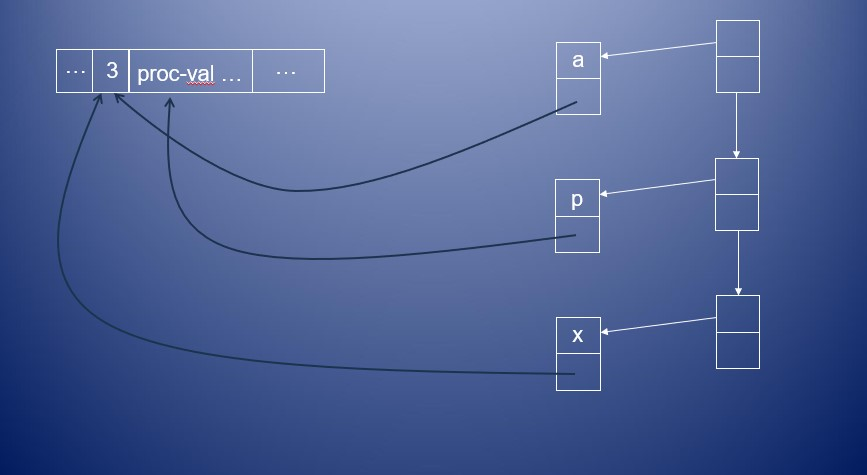
\includegraphics[scale=0.5]{cbr3.jpg}
\end{center}

\end{itemize}
\end{scriptsize}
\end{frame}

\begin{frame}[fragile]
\frametitle{Parameter Passing Variations}
\framesubtitle{Call by Reference}
\begin{scriptsize}
\begin{itemize}
\item<1->
\begin{alltt}
let a = 3
	p = proc (x) \textcolor{red}{set x = 4}
in begin
    (p a);
    a
   end
\end{alltt}

\item<1->
\begin{center}
  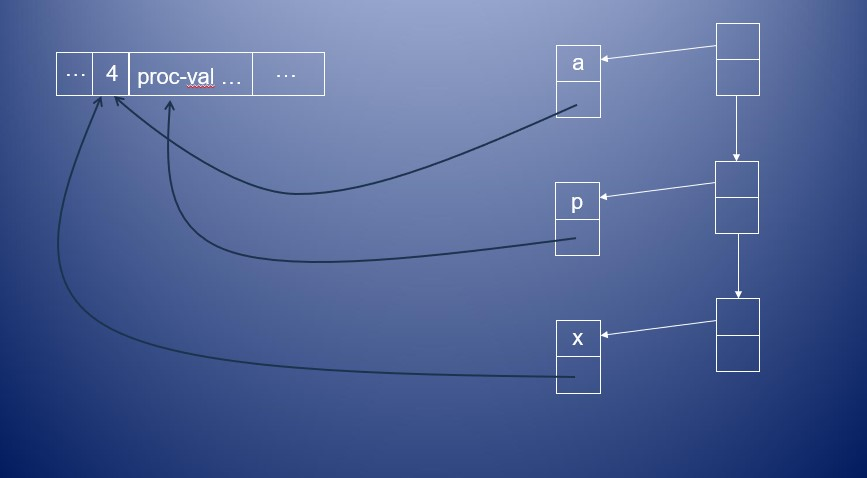
\includegraphics[scale=0.5]{cbr4.jpg}
\end{center}

\item<1-> Returns 4

\end{itemize}
\end{scriptsize}
\end{frame}

\begin{frame}[fragile]
\frametitle{Parameter Passing Variations}
\framesubtitle{Call by Reference}
\begin{scriptsize}
\begin{itemize}
\item<1-> Why use call-by-reference?
\begin{itemize}
\item[\arrow] Return multiple values (by making assignments to parameters)

\item[\arrow] Implementation of common operations
\end{itemize}


\end{itemize}
\end{scriptsize}
\end{frame}

\begin{frame}[fragile]
\frametitle{Parameter Passing Variations}
\framesubtitle{Call by Reference}
\begin{scriptsize}
\begin{itemize}
\item<1-> Call-by-Value
\begin{alltt}
\begin{tiny}
let \textcolor{red}{a = 3
    b = 4
    swap = proc (x, y)
	        let temp = x
	        in begin
	             set x = y
	             set y = temp
	           end}
in begin
     swap(a b)
     -(a, b)
   end
\end{tiny}
\end{alltt}

\item<1->
\begin{center}
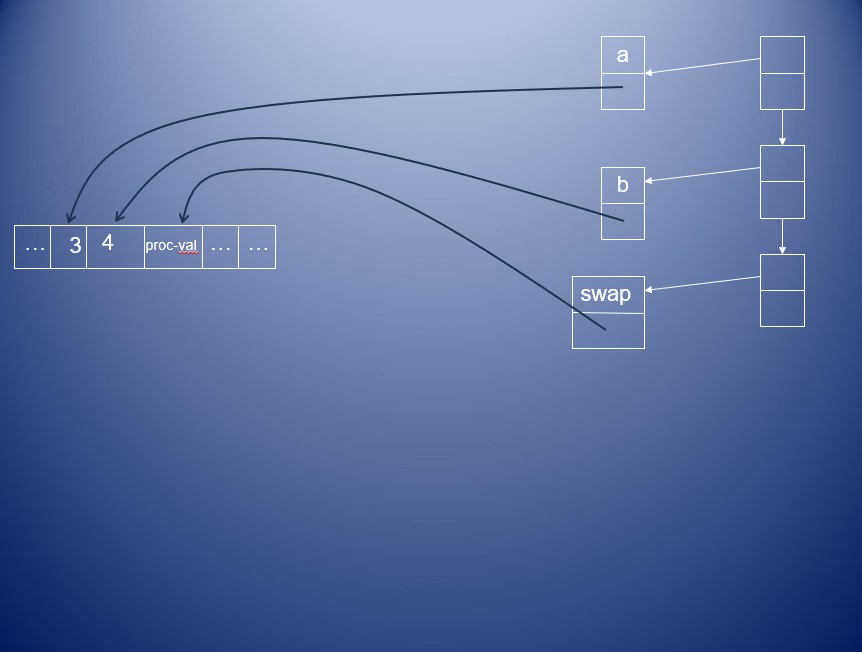
\includegraphics[scale=0.35]{cbv-cbr1.jpg}
\end{center}

\end{itemize}
\end{scriptsize}
\end{frame}

\begin{frame}[fragile]
\frametitle{Parameter Passing Variations}
\framesubtitle{Call by Reference}
\begin{scriptsize}
\begin{itemize}
\item<1-> Call-by-Value
\begin{alltt}
\begin{tiny}
let a = 3
    b = 4
    swap = proc (x, y)
	        let temp = x
	        in begin
	             set x = y
	             set y = temp
	           end
in begin
     \textcolor{red}{swap(a b)}
     -(a, b)
   end
\end{tiny}
\end{alltt}

\item<1->
\begin{center}
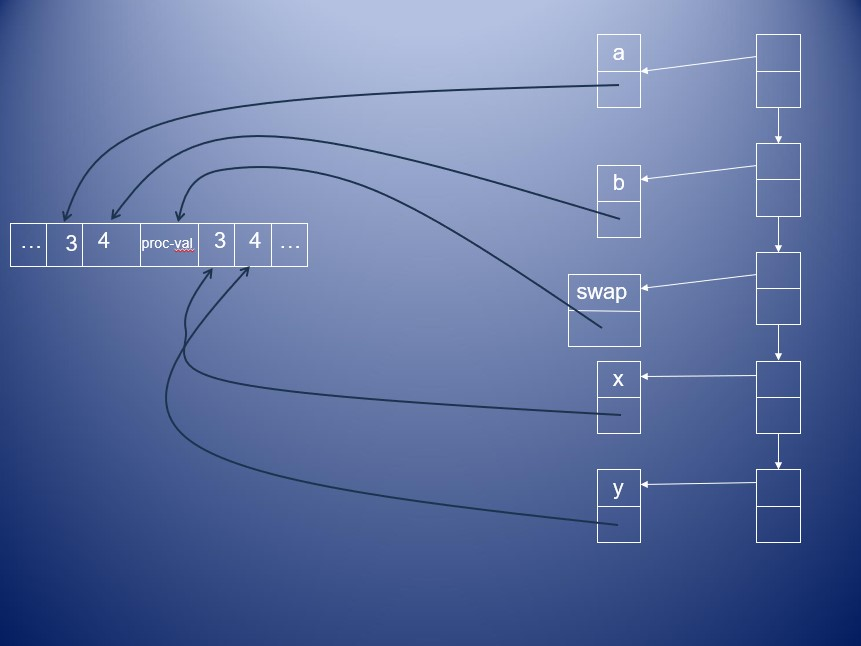
\includegraphics[scale=0.35]{cbv-cbr2.jpg}
\end{center}

\end{itemize}
\end{scriptsize}
\end{frame}

\begin{frame}[fragile]
\frametitle{Parameter Passing Variations}
\framesubtitle{Call by Reference}
\begin{scriptsize}
\begin{itemize}
\item<1-> Call-by-Value
\begin{alltt}
\begin{tiny}
let a = 3
    b = 4
    swap = proc (x, y)
	        \textcolor{red}{let temp = x}
	        in begin
	             set x = y
	             set y = temp
	           end
in begin
     swap(a b)
     -(a, b)
   end
\end{tiny}
\end{alltt}

\item<1->
\begin{center}
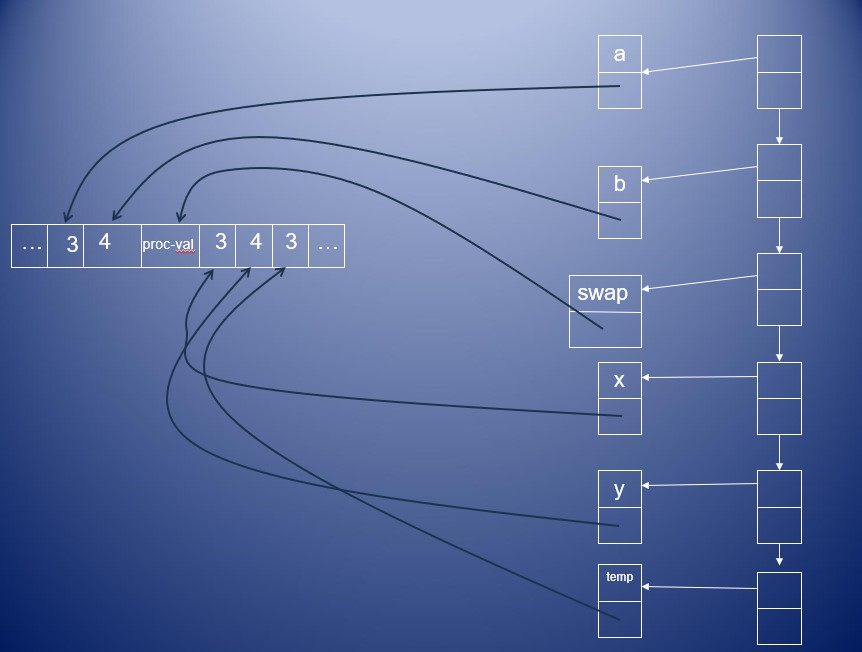
\includegraphics[scale=0.35]{cbv-cbr3.jpg}
\end{center}

\end{itemize}
\end{scriptsize}
\end{frame}

\begin{frame}[fragile]
\frametitle{Parameter Passing Variations}
\framesubtitle{Call by Reference}
\begin{scriptsize}
\begin{itemize}
\item<1-> Call-by-Value
\begin{alltt}
\begin{tiny}
let a = 3
    b = 4
    swap = proc (x, y)
	        let temp = x
	        in begin
	             \textcolor{red}{set x = y}
	             set y = temp
	           end
in begin
     swap(a b)
     -(a, b)
   end
\end{tiny}
\end{alltt}

\item<1->
\begin{center}
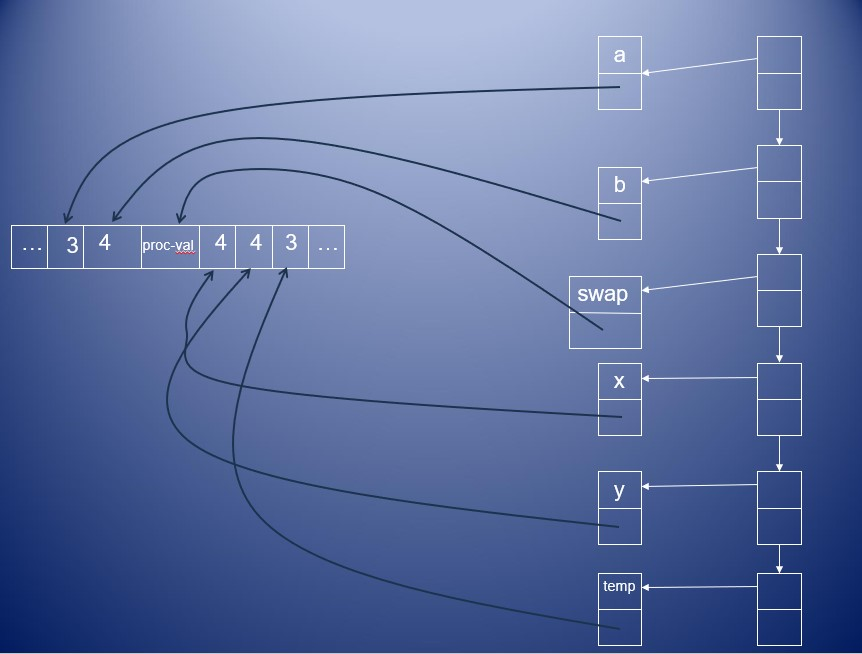
\includegraphics[scale=0.35]{cbv-cbr4.jpg}
\end{center}

\end{itemize}
\end{scriptsize}
\end{frame}

\begin{frame}[fragile]
\frametitle{Parameter Passing Variations}
\framesubtitle{Call by Reference}
\begin{scriptsize}
\begin{itemize}
\item<1-> Call-by-Value
\begin{alltt}
\begin{tiny}
let a = 3
    b = 4
    swap = proc (x, y)
	        let temp = x
	        in begin
	             set x = y
	             \textcolor{red}{set y = temp}
	           end
in begin
     swap(a b)
     -(a, b)
   end                            \begin{normalsize} \textcolor{darkgreen}{Returns -1} \end{normalsize}
\end{tiny}
\end{alltt}

\item<1->
\begin{center}
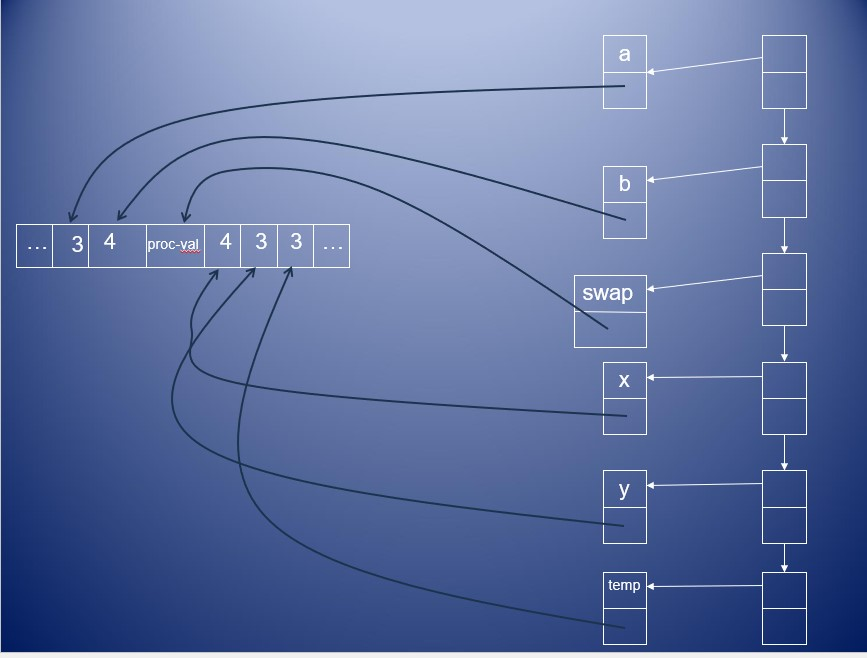
\includegraphics[scale=0.35]{cbv-cbr5.jpg}
\end{center}


\end{itemize}
\end{scriptsize}
\end{frame}

\begin{frame}[fragile]
\frametitle{Parameter Passing Variations}
\framesubtitle{Call by Reference}
\begin{scriptsize}
\begin{itemize}
\item<1-> Call-by-Reference
\begin{alltt}
\begin{tiny}
let \textcolor{red}{a = 3
    b = 4
    swap = proc (x, y)
	        let temp = x}
	        in begin
	             set x = y
	             set y = temp
	           end
in begin
     \textcolor{red}{swap(a b)}
     -(a, b)
   end
\end{tiny}
\end{alltt}

\item<1->
\begin{center}
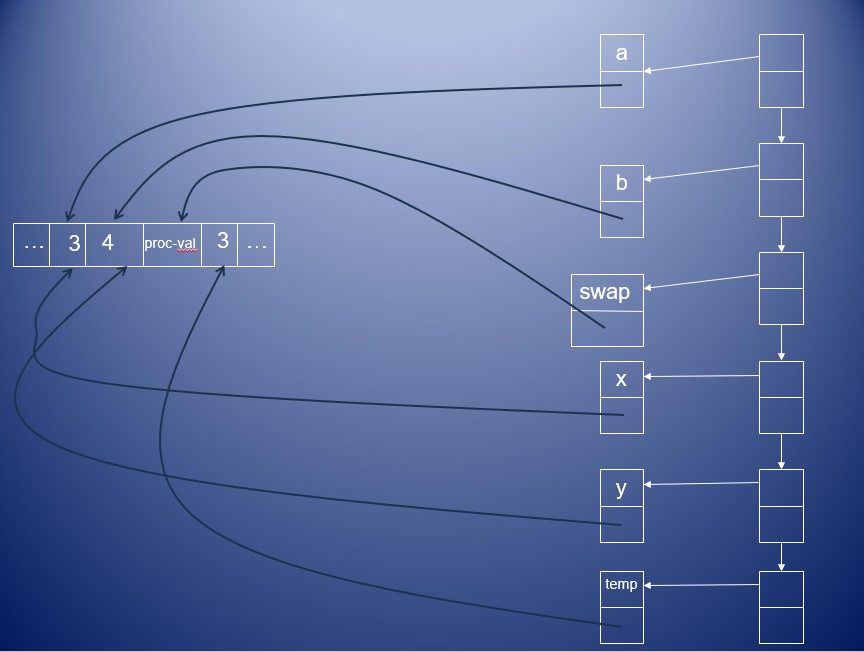
\includegraphics[scale=0.35]{cbv-cbr6.jpg}
\end{center}

\end{itemize}
\end{scriptsize}
\end{frame}

\begin{frame}[fragile]
\frametitle{Parameter Passing Variations}
\framesubtitle{Call by Reference}
\begin{scriptsize}
\begin{itemize}
\item<1-> Call-by-Reference
\begin{alltt}
\begin{tiny}
let a = 3
    b = 4
    swap = proc (x, y)
	        let temp = x
	        in begin
	             \textcolor{red}{set x = y}
	             set y = temp
	           end
in begin
     swap(a b)
     -(a, b)
   end
\end{tiny}
\end{alltt}

\item<1->
\begin{center}
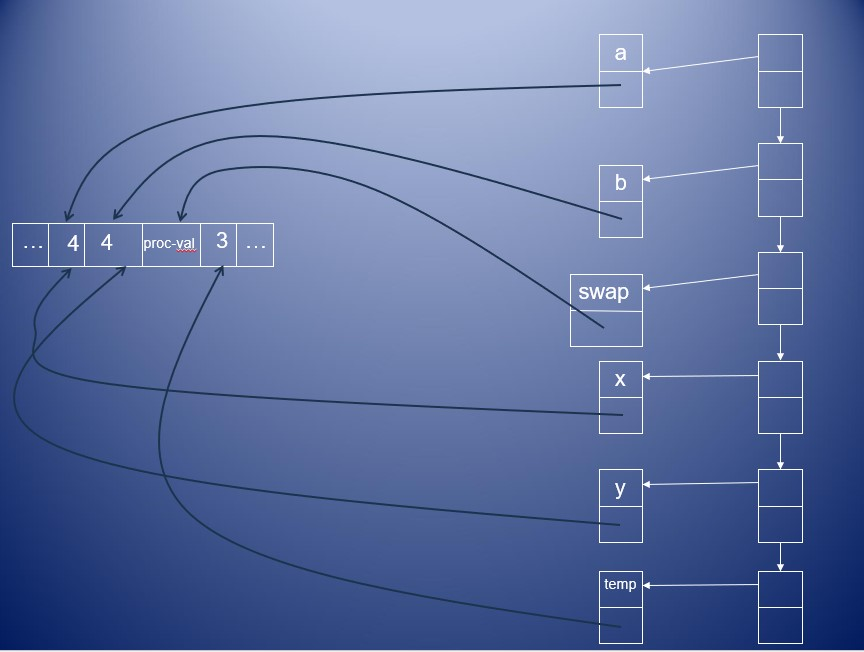
\includegraphics[scale=0.35]{cbv-cbr7.jpg}
\end{center}

\end{itemize}
\end{scriptsize}
\end{frame}

\begin{frame}[fragile]
\frametitle{Parameter Passing Variations}
\framesubtitle{Call by Reference}
\begin{scriptsize}
\begin{itemize}
\item<1-> Call-by-Reference
\begin{alltt}
\begin{tiny}
let a = 3
    b = 4
    swap = proc (x, y)
	        let temp = x
	        in begin
	             set x = y
	             \textcolor{red}{set y = temp}
	           end
in begin
     swap(a b)
     -(a, b)
   end                            \begin{normalsize} \textcolor{darkgreen}{Returns 1} \end{normalsize}
\end{tiny}
\end{alltt}

\item<1->
\begin{center}
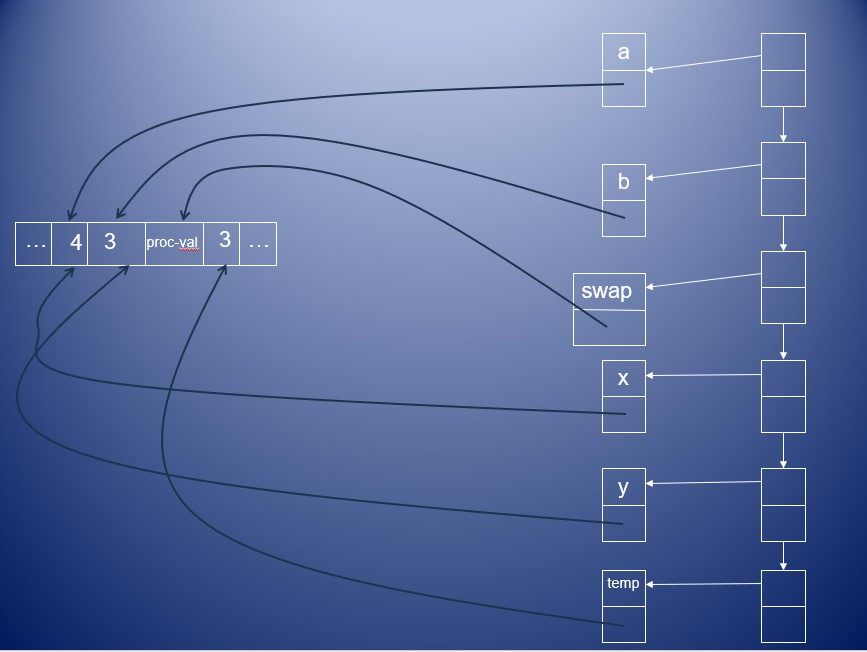
\includegraphics[scale=0.35]{cbv-cbr8.jpg}
\end{center}

\end{itemize}
\end{scriptsize}
\end{frame}



\begin{frame}[fragile]
\frametitle{Parameter Passing Variations}
\framesubtitle{Call by Reference}
\begin{scriptsize}
\begin{itemize}
\item<1-> Only change is for when new references are created:
\begin{itemize}
 \item[\arrow] call-by-value: a new reference is created for every operand evaluated

 \item[\arrow] call-by-reference: a new reference is created for evaluation of an operand other than a variable
\end{itemize}

\item Under call-by-reference we need a new location for some operands and not for others

\end{itemize}
\end{scriptsize}
\end{frame}

\begin{frame}[fragile]
\frametitle{Parameter Passing Variations}
\framesubtitle{Call by Reference}
\begin{scriptsize}
\begin{itemize}
\item<1->
\begin{alltt}
;; apply-procedure : proc (listof expval) -> expval
(define (apply-procedure f vals)
  (cases proc f
    (procedure (params body envv)
      (let [(saved-env (vector-ref envv 0))]
        (value-of body
          (foldr (lambda (binding acc)
                   (extend-env (car binding)
                               (newref (cadr binding))
                               acc))
                 saved-env
                 (map (lambda (p v) (list p v)) params vals)))))))
\textcolor{red}{Can't always allocate an argument in the store}
\end{alltt}

\item<2->
\begin{alltt}
;; apply-procedure : proc \textcolor{red}{(listof ref)} -> expval
(define (apply-procedure f vals)
 (cases proc f
  (procedure (params body envv)
   (let [(saved-env (vector-ref envv 0))]
    (value-of body
             (foldr (lambda (binding acc)
                     (extend-env (car binding) (cadr binding) acc))
                     saved-env
                     (map (lambda (p v) (list p v)) params vals)))))))
\textcolor{red}{Decision made in the evaluation of a call-exp}
\end{alltt}

\end{itemize}
\end{scriptsize}
\end{frame}

\begin{frame}[fragile]
\frametitle{Parameter Passing Variations}
\framesubtitle{Call by Reference}
\begin{scriptsize}
\begin{itemize}
\item<1-> In value-of
\begin{alltt}
(call-exp (rator rands)
  (let [(proc (expval2proc (value-of rator env)))
        (args (map (lambda (rand) (value-of rand env)) rands))]
    (apply-procedure proc args)))

\textcolor{red}{apply-procedure must be called with a (listof ref)}
\end{alltt}

\item<2->
\begin{alltt}
(call-exp (rator rands)
  (let [(proc (expval2proc (value-of rator env)))
        (args (map (lambda (rand) (value-of-rand rand env)) rands))]
    (apply-procedure proc args)))

\textcolor{red}{value-of-rand returns a reference}
\end{alltt}

\item<3->
\begin{alltt}
;; value-of-rand : expression environment -> Ref
;; Purpose: For a var-exp return existing reference.
;;          Otherwise, return reference to a new cell.
(define (value-of-rand exp env)
  (cases expression exp
    (var-exp (var) (apply-env env var))
    (else (newref (value-of exp env)))))
\end{alltt}

\end{itemize}
\end{scriptsize}
\end{frame}

\begin{frame}[fragile]
\frametitle{Parameter Passing Variations}
\framesubtitle{Call by Reference}
\begin{scriptsize}
\begin{itemize}
\item<1->
\begin{alltt}
(check-equal? (eval "let a = 3
                     in let p = proc (x) set x = 4
                        in begin (p a); a end")
              (num-val 4))
(check-equal? (eval "let x = 0
                     in letrec f (x) = set x = +(x, 1)
                               g (a) = set x = +(x, 2)
                        in begin (f x);
                                 (g x);
                                 x
                           end")
              (num-val 3))
(check-equal?
 (eval "let swap = proc (a)
                    proc (b)
                      let t = a
                      in begin set a = b;  set b = t  end
        in let a = 33
           in let b = 44
              in begin ((swap a) b);
                       -(a, b)
                 end")
 (num-val 11))
\end{alltt}

\end{itemize}
\end{scriptsize}
\end{frame}


\begin{frame}[fragile]
\frametitle{Parameter Passing Variations}
\framesubtitle{Lazy Evaluation: Call by Name}
\begin{scriptsize}
\begin{itemize}
\item<1-> Call-by-value and call-by-reference are eager

\item<1-> Always find the value of each operand

\item<2-> Lazy evaluation

\item<2-> Operands not evaluated until needed

\item<2-> Never needed \arrow{} never evaluated

\item<3-> Is this useful?


\end{itemize}
\end{scriptsize}
\end{frame}

\begin{frame}[fragile]
\frametitle{Parameter Passing Variations}
\framesubtitle{Lazy Evaluation: Call by Name}
\begin{scriptsize}
\begin{itemize}
\item<1-> 
\begin{alltt}
letrec compute-ints-from-n (n) = (compute-ints-from-n +(n, 1))
in let f = proc (k) 42
   in (f (compute-ints-from-n 100))
\end{alltt}

\item<1-> What should this program return?

\item<2-> It should return 42, but does not. Why?

\item<3-> Under lazy evaluation this program returns 42

\item<4->
\begin{alltt}
#lang eopl
(require rackunit "../eopl-extras.rkt")

(define (ints-from n) (stream-cons n (ints-from (+ n 1))))
(define natnums (ints-from 0))
(define (nth-natnum n) (stream-ref natnums n))
(define (first-n-natnums n)
  (if (= n 0)
      (list (nth-natnum 0))
      (cons (nth-natnum n) (first-n-natnums (- n 1)))))

(check-equal?  (first-n-natnums 10)
               \quot{}(10 9 8 7 6 5 4 3 2 1 0))
(check-equal?  (first-n-natnums 15)
               \quot{}(15 14 13 12 11 10 9 8 7 6 5 4 3 2 1 0))
\end{alltt}


\end{itemize}
\end{scriptsize}
\end{frame}

\begin{frame}[fragile]
\frametitle{Parameter Passing Variations}
\framesubtitle{Lazy Evaluation: Call by Name}
\begin{scriptsize}
\begin{itemize}
\item<1->
\begin{alltt}
#lang eopl
(require rackunit "../eopl-extras.rkt")

;; natnum --> natnum
;; Purpose: Return the kth Fibonacci number
(define (fib k)
  (if (< k 2)
      1
      (+ (fib (- k 1)) (fib (- k 2)))))
(define (the-fibs n) (stream-cons (fib n) (the-fibs (+ n 1))))
(define fibs (the-fibs 0))
(define (nth-fib n) (stream-ref fibs n))

(check-equal?  (nth-fib 5)  8)
(check-equal?  (nth-fib 10) 89)
\end{alltt}

\item<2->
\begin{alltt}
(define the-doubles (stream-map (\(\lambda\) (n) (* 2 n)) natnums))

(check-equal? (stream-ref the-doubles 10) 20)
(check-equal? (stream-ref the-doubles 1287) 2574)
\end{alltt}

\end{itemize}
\end{scriptsize}
\end{frame}

\begin{frame}[fragile]
\frametitle{Parameter Passing Variations}
\framesubtitle{Lazy Evaluation: Call by Name}
\begin{scriptsize}
\begin{itemize}
\item<1-> An operand is not evaluated until needed

\item<2-> A bound var is associated with unevaluated  expression (frozen)

\item<3-> When the value of the bound var is needed, then the expression is evaluated (thawed)

\item<4-> What does this require?

\item<5-> The env that exists when the expr is frozen

\item<6->
\begin{alltt}
(define-datatype thunk thunk?
  (a-thunk
    (exp1 expression?)
    (env environment?)))
\end{alltt}

\item<6-> The expr in a thunk is evaluated when a proc needs the value of bound var


\end{itemize}
\end{scriptsize}
\end{frame}

\begin{frame}[fragile]
\frametitle{Parameter Passing Variations}
\framesubtitle{Lazy Evaluation: Call by Name}
\begin{scriptsize}
\begin{itemize}

\item<1-> Language
\begin{itemize}
  \item[\arrow] let remains eager
  \item[\arrow] lazy evaluation of arguments
  \item[\arrow] effects
\end{itemize}

\item<2-> Values
\begin{itemize}
  \item[\arrow] expval = int + bool + proc
  \item[\arrow] denval = ref(expval + thunk)
\end{itemize}

\item<3-> New allocations policy
\begin{itemize}
  \item[\arrow] var: pass its denotation (which is a reference; same as call-by-reference)
  \item[\arrow] not var: pass a ref to a new location storing a thunk for the unevaluated arg
\end{itemize}

\end{itemize}
\end{scriptsize}
\end{frame}

\begin{frame}[fragile]
\frametitle{Parameter Passing Variations}
\framesubtitle{Lazy Evaluation: Call by Name}
\begin{scriptsize}
\begin{itemize}
\item<1-> 
\begin{alltt}
;; value-of-rand : expression environment -> Ref
;; Purpose: if the expression is a var-exp, then return the reference.
;; otherwise,return a thunk for the given expression.
(define (value-of-rand exp env)
  (cases expression exp
    (var-exp (var) (apply-env env var))
    (else
     (newref (a-thunk exp env))))) \textcolor{red}{\(\leftarrow\) not a var-exp create thunk}
\end{alltt}

\end{itemize}
\end{scriptsize}
\end{frame}

\begin{frame}[fragile]
\frametitle{Parameter Passing Variations}
\framesubtitle{Lazy Evaluation: Call by Name}
\begin{scriptsize}
\begin{itemize}
\item<1-> How do you evaluate a var-expr?

\item<2->
$\frac{w \ = \ deref(\rho(v))}{(value\text{-}of \ (var\text{-}exp v) \ \rho) \ = \ \textrm{if (expval? w) then w else  (value-of-thunk w)}
}$

\item<3-> change to value-of
\begin{alltt}
(var-exp (var)
  (let ((ref1 (apply-env env var)))
    (let ((w (deref ref1)))
      (if (expval? w)
          w					
		  (value-of-thunk w))))
\end{alltt}

\end{itemize}
\end{scriptsize}
\end{frame}

\begin{frame}[fragile]
\frametitle{Parameter Passing Variations}
\framesubtitle{Lazy Evaluation: Call by Name}
\begin{scriptsize}
\begin{itemize}

\item<1-> Evaluating a thunk
\begin{alltt}
;; value-of-thunk : thunk -> expval
;; Purpose: Evaluate the given thunk
(define (value-of-thunk th)
  (cases thunk th
    (a-thunk (exp1 saved-env)
             (value-of exp1 saved-env))))
\end{alltt}

\end{itemize}
\end{scriptsize}
\end{frame}

\begin{frame}[fragile]
\frametitle{Parameter Passing Variations}
\framesubtitle{Lazy Evaluation: Call by Name}
\begin{scriptsize}
\begin{itemize}
\item<1-> Consider
\begin{alltt}
let g = let counter = 10
            in proc (d) *(2, counter)
in (proc (x) +(x, x) (g 0))
\end{alltt}

\item<2-> x is the thunk for (g 0)

\item<3-> the first x forces the evaluation of the thunk \arrow{} 20

\item<4-> the second x forces the evaluation of the thunk \arrow{} 20

\item<4-> returns 40
\end{itemize}
\end{scriptsize}
\end{frame}


\begin{frame}[fragile]
\frametitle{Parameter Passing Variations}
\framesubtitle{Lazy Evaluation: Call by Need}
\begin{scriptsize}
\begin{itemize}
\item<1-> Evaluating the same thunk seems wasteful

\item<2-> Solution: Evaluate it once and mutate it for its value

\item<3-> Change in value-of
\begin{alltt}
(var-exp (var)
  (let ((ref1 (apply-env env var)))
    (let ((w (deref ref1)))
      (if (expval? w)
          w	
          (let ((v1 (value-of-thunk w)))
            (begin
              (setref! ref1 v1)
              v1))))))
\end{alltt}

\end{itemize}
\end{scriptsize}
\end{frame}

\begin{frame}[fragile]
\frametitle{Parameter Passing Variations}
\framesubtitle{Lazy Evaluation: Call by Need}
\begin{scriptsize}
\begin{itemize}
\item<1-> Change how var-exp are evaluated
\begin{alltt}
(var-exp (var)
  (let ((ref1 (apply-env env var)))
    (let ((w (deref ref1)))
      (if (expval? w)
          w	
          (let ((v1 (value-of-thunk w)))
            (begin
              (setref! ref1 v1)
              v1))))))
\end{alltt}

\end{itemize}
\end{scriptsize}
\end{frame}

\begin{frame}[fragile]
\frametitle{Parameter Passing Variations}
\framesubtitle{Lazy Evaluation: Call by Need}
\begin{scriptsize}
\begin{itemize}
\item<1-> 
\begin{alltt}
let g = let counter = 10
        in proc (d) *(2, counter)
in (proc (x) +(x, x) (g 0))
\end{alltt}

\item<2> x is the thunk for (g 0)

\item<3-> the first x forces the evaluation of the thunk to 20 

\item<3-> mutates x to 20

\item<4-> the second x (simply) returns its value of 20

\item<4-> returns 40


\end{itemize}
\end{scriptsize}
\end{frame}

\begin{frame}[fragile]
\frametitle{Parameter Passing Variations}
\framesubtitle{Lazy Evaluation: Call by Need}
\begin{scriptsize}
\begin{itemize}
\item<1-> In the absence of side-effects, call-by-name and call-by-need always yield the same answer

\item<2-> In the presence of side-effects, it is easy to distinguish them

\item<3->
\begin{alltt}
let g = let count = 0
        in proc (d)
	         begin
               set count = incr(count);
               count
	       end
in (proc (x) +(x, x) (g 0) )
\end{alltt}

\item<4-> g returns the number of times it is called

\item<4-> Thunk for (g 0) is passed as the argument to the function in the body of the let

\item<5-> call-by-name

\item<6-> the first reference to x: sets count to 1 \& returns 1 as the value of (g 0)

\item<7-> the second reference to x: sets count to 2 \& returns 2 as the value of (g 0)

\item<8-> +(1, 2) = 3

\item<9-> call-by-need

\item<10-> the first reference to x forces: sets count to 1, returns 1 as the value of (g 0), and stores 1 as the value of (g 0)
\item<11-> second reference to x: returns the stored 1 

\item<12>  +(1, 1) = 2

\end{itemize}
\end{scriptsize}
\end{frame}

\begin{frame}[fragile]
\frametitle{Parameter Passing Variations}
%\framesubtitle{Lazy Evaluation: Call by Need}
\begin{scriptsize}
\begin{itemize}
\item<1-> Lazy evaluation: in the absence of side-effects allows for a simple way to reason about programs

\item<2-> The effect of a procedure call is modeled by:
\begin{itemize}
 \item[\arrow] Replacing the call with the body of the procedure
 \item[\arrow] Every reference to a parameter in the body is replaced by the corresponding operand
 \item[\arrow]This evaluation strategy is the basis of the lambda calculus and is known as $\beta$-reduction
\end{itemize}

\item<3-> $\beta$-reduction: $\lambda$(x.e)x0 \arrow{} e\{x0/x\}
\begin{alltt}
\(\lambda\)(x.+(x, *(2, x)) -(5, -10)
\arrow{} +(-(5, -10) *(2, -(5, -10)))
\arrow{} +(15, *(2, -(5, -10)))
\arrow{} +(15, *(2, 15))
\arrow{} +(15, 30)
\arrow{} 45
\end{alltt}

\end{itemize}
\end{scriptsize}
\end{frame}

\begin{frame}[fragile]
\frametitle{Parameter Passing Variations}
%\framesubtitle{Lazy Evaluation: Call by Need}
\begin{scriptsize}
\begin{itemize}
\item<1-> All the freezing and thawing can lead to considerable overhead

\item<1-> Reducing the number of thunks created is important for efficiency

\item<2-> Difficult to determine the order of evaluation which is essential for programs with side-effects

\item<3-> You do not have to think operationally: you can reason equationally about your programs.-–S. Doaitse Swierstra
\item<3-> I prefer call by value to call by name because it is more predictable.-–Mitchell Wand

\item<4-> Popular with pure functional languages (i.e. with no side-effects) and rarely found elsewhere
    
\item<4-> Haskell and Clean	
		
\item<4-> C\# (deferred execution)

\end{itemize}
\end{scriptsize}
\end{frame}

\begin{frame}[fragile]
\frametitle{Parameter Passing Variations}
%\framesubtitle{Lazy Evaluation: Call by Need}
\begin{scriptsize}
\begin{itemize}
\item<1-> HOMEWORK: 4.31, 4.32, 4.39, 4.40, 4.42

\end{itemize}
\end{scriptsize}
\end{frame}

\end{document} 